% Options for packages loaded elsewhere
\PassOptionsToPackage{unicode}{hyperref}
\PassOptionsToPackage{hyphens}{url}
%
\documentclass[
  10pt,
]{article}
\usepackage{lmodern}
\usepackage{amssymb,amsmath}
\usepackage{ifxetex,ifluatex}
\ifnum 0\ifxetex 1\fi\ifluatex 1\fi=0 % if pdftex
  \usepackage[T1]{fontenc}
  \usepackage[utf8]{inputenc}
  \usepackage{textcomp} % provide euro and other symbols
\else % if luatex or xetex
  \usepackage{unicode-math}
  \defaultfontfeatures{Scale=MatchLowercase}
  \defaultfontfeatures[\rmfamily]{Ligatures=TeX,Scale=1}
\fi
% Use upquote if available, for straight quotes in verbatim environments
\IfFileExists{upquote.sty}{\usepackage{upquote}}{}
\IfFileExists{microtype.sty}{% use microtype if available
  \usepackage[]{microtype}
  \UseMicrotypeSet[protrusion]{basicmath} % disable protrusion for tt fonts
}{}
\makeatletter
\@ifundefined{KOMAClassName}{% if non-KOMA class
  \IfFileExists{parskip.sty}{%
    \usepackage{parskip}
  }{% else
    \setlength{\parindent}{0pt}
    \setlength{\parskip}{6pt plus 2pt minus 1pt}}
}{% if KOMA class
  \KOMAoptions{parskip=half}}
\makeatother
\usepackage{xcolor}
\IfFileExists{xurl.sty}{\usepackage{xurl}}{} % add URL line breaks if available
\IfFileExists{bookmark.sty}{\usepackage{bookmark}}{\usepackage{hyperref}}
\hypersetup{
  pdftitle={Relazione progetto Programmazione a Oggetti A.A. 2019/20},
  pdfauthor={Gabriel Bizzo - 1170734, Marco Rosin - 1120673, Andrea Moscon - 1121217},
  hidelinks,
  pdfcreator={LaTeX via pandoc}}
\urlstyle{same} % disable monospaced font for URLs
\usepackage{graphicx}
\makeatletter
\def\maxwidth{\ifdim\Gin@nat@width>\linewidth\linewidth\else\Gin@nat@width\fi}
\def\maxheight{\ifdim\Gin@nat@height>\textheight\textheight\else\Gin@nat@height\fi}
\makeatother
% Scale images if necessary, so that they will not overflow the page
% margins by default, and it is still possible to overwrite the defaults
% using explicit options in \includegraphics[width, height, ...]{}
\setkeys{Gin}{width=\maxwidth,height=\maxheight,keepaspectratio}
% Set default figure placement to htbp
\makeatletter
\def\fps@figure{htbp}
\makeatother
\setlength{\emergencystretch}{3em} % prevent overfull lines
\providecommand{\tightlist}{%
  \setlength{\itemsep}{0pt}\setlength{\parskip}{0pt}}
\setcounter{secnumdepth}{-\maxdimen} % remove section numbering
\ifluatex
  \usepackage{selnolig}  % disable illegal ligatures
\fi

\title{Relazione progetto Programmazione a Oggetti A.A. 2019/20}
\author{Gabriel Bizzo - 1170734 \\ \and Marco Rosin - 1120673 \\ \and Andrea Moscon - 1121217}
\date{Relazione di Rosin Marco}

\begin{document}
\maketitle

\begin{center}
  
\includegraphics[width=0.5\textwidth,height=\textheight]{./logo.png}
\end{center}
\begin{center}
  
\includegraphics[width=0.75\textwidth,height=\textheight]{./Logo-DM.png}
\end{center}

\newpage

\hypertarget{abstract-e-funzionalituxe0}{%
\section{Abstract e Funzionalità}\label{abstract-e-funzionalituxe0}}

Lo scopo del progetto è fornire un applicativo per informatizzare una
pizzeria da asporto ecologica e orientata ai prodotti locali,
implementando una gestione efficiente di inventario, menu e comande.

L'applicativo fornisce all'utente le seguenti funzionalità:

\begin{itemize}
\tightlist
\item
  Inserimento, rimozione e modifica di un articolo dal menù
\item
  Inserimento, rimozione e modifica (in modo \emph{smart}) di un
  ingrediente dall'inventario.
\item
  Inserimento, rimozione e modifica (in modo \emph{smart}) di una
  comanda da una bacheca apposita.
\item
  Una funzionalità di \emph{contabilizzazione} per calcolare il
  guadagno/perdita della pizzeria in un determinato periodo di tempo.
\item
  Una funzionalità di salvataggio e caricamento di tutti i dati del
  programma.
\end{itemize}

\hypertarget{progettazione-e-descrizione-delle-gerarchie-utilizzate}{%
\section{Progettazione e descrizione delle gerarchie
utilizzate}\label{progettazione-e-descrizione-delle-gerarchie-utilizzate}}

\hypertarget{gerarchia-g}{%
\subsection{Gerarchia G}\label{gerarchia-g}}

\begin{figure}
\centering
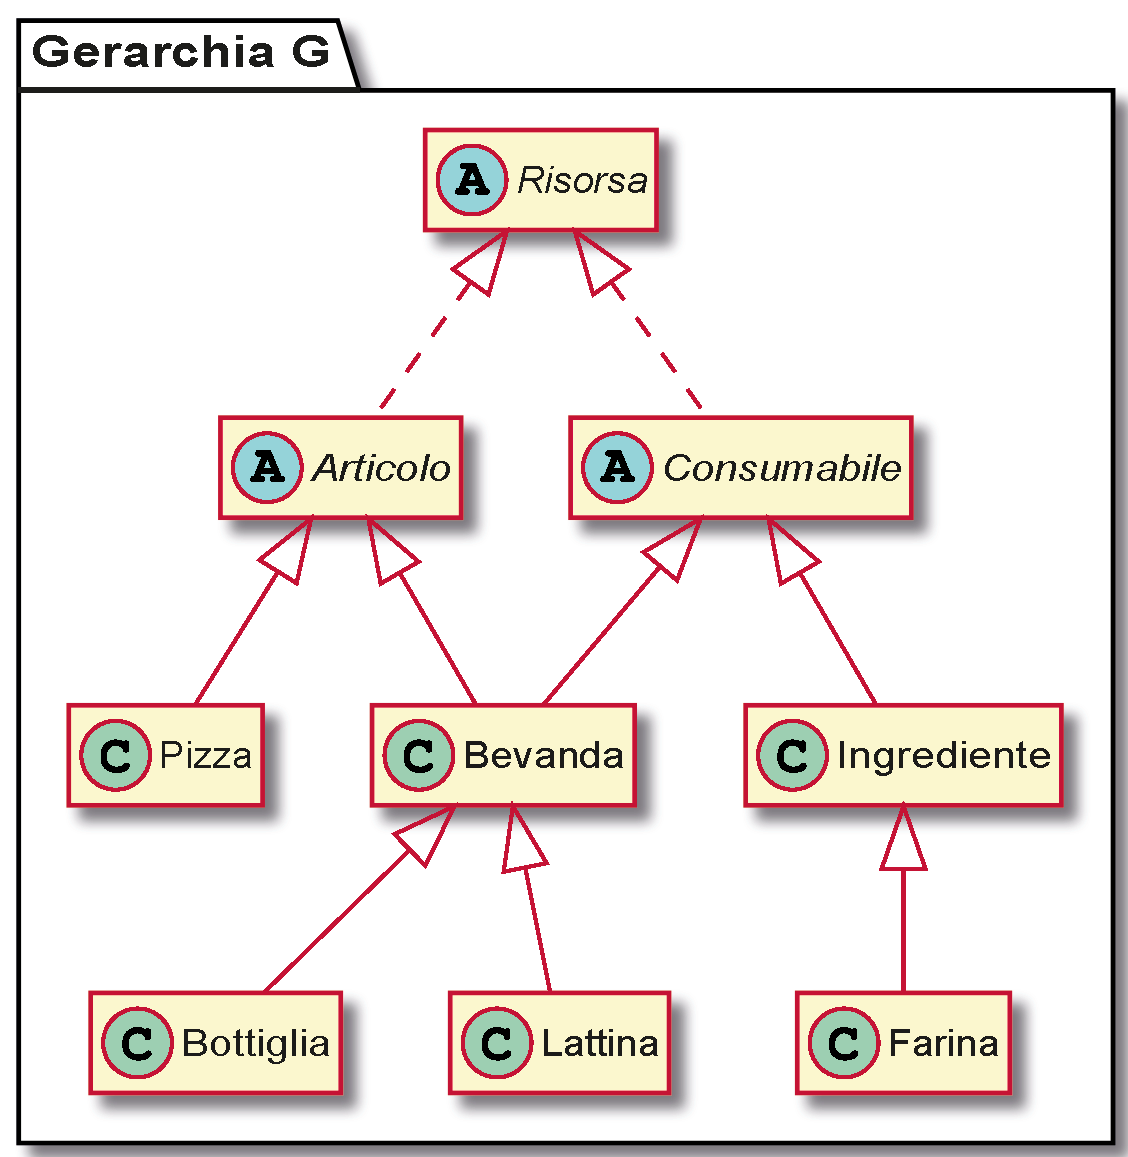
\includegraphics[width=0.6\textwidth,height=\textheight]{./gerarchiaG.png}
\caption{gerarchia G}
\end{figure}
\newpage
\begin{itemize}
\item
  \texttt{Risorsa}: Base astratta della gerarchia, rappresenta ad alto
  livello ogni elemento gestito dalla pizzeria. Contiene informazioni
  generiche di ogni oggetto (ID, nome, disponibilità) e definisce dei
  metodi virtuali puri da implementare nelle sottoclassi concrete.
\item
  \texttt{Articolo}: Sottotipo astratto derivante da \texttt{Risorsa},
  le cui istanze rappresentano i prodotti venduti dalla pizzeria.
  Aggiunge l'informazione relativa al prezzo iniziale di ogni articolo
  venduto e due metodi virtuali puri che ritornano rispettivamente il
  prezzo e la composizione di ogni articolo.
\item
  \texttt{Consumabile}: Sottotipo astratto derivante da
  \texttt{Risorsa}, rappresenta gli oggetti di consumo usati dalla
  pizzeria per preparare gli articoli da vendere. Aggiunge i campi dati
  quantità acquistata, costo e data d'acquisto necessari per il calcolo
  della contabilizzazione e un metodo virtuale puro che ritorna la spesa
  sostenuta dalla pizzeria per acquistare un consumabile
\item
  \texttt{Pizza}: Sottotipo concreto derivante da \texttt{Articolo}, le
  cui istanze rappresentano le pizze presenti nel menu della pizzeria.
  Implementa i metodi virtuali ereditati da \texttt{Articolo} per
  calcolare il prezzo d'acquisto e la lista di ingredienti usati nella
  pizza.
\item
  \texttt{Bevanda}: Sottotipo concreto derivante da \texttt{Articolo} e
  \texttt{Consumabile}, che implementa i metodi virtuali puri di
  entrambe le superclassi.
\item
  \texttt{Ingrediente}: Sottotipo concreto derivante da
  \texttt{Consumabile}, le cui istanze rappresentano gli ingredienti
  usati dalla pizzeria per creare le pizze. Aggiunge il booleano
  \emph{locale}, che indica la provenienza dell'ingrediente (gli
  ingredienti locali hanno un costo d'acquisto maggiore, che si riflette
  in un prezzo più alto per gli articoli che lo usano). Implementa il
  metodo virtuale ereditato da \texttt{Consumabile} per calcolare il
  costo d'acquisto.
\item
  \texttt{Bottiglia}, \texttt{Lattina}: Sottotipi concreti derivanti da
  \texttt{Bevanda}, le cui istanze rappresentano un tipo particolare di
  bevanda (indicato dal nome della classe). Si è scelto di differenziare
  in questo modo i diversi tipi di bevanda per aumentare l'estensibilità
  del modello, in quanto per aggiungere nuove tipologie di bevanda è
  sufficiente estendere la classe \texttt{Bevanda}.
\item
  \texttt{Farina}: Sottotipo concreto derivante da \texttt{Ingrediente},
  le cui istanze rappresentano le diverse farine usate dalla pizzeria
  per preparare le pizze. In quanto particolare tipo di ingrediente non
  implementa i metodi virtuali ereditati da \texttt{Consumabile} ma
  sfrutta le implementazioni della superclasse. Si è scelto di
  differenziare in questo modo i diversi tipi di farina per aumentare
  l'estensibilità del modello, in quanto per aggiungere nuove farine è
  sufficiente creare nuove istanze di questa classe.
\end{itemize}
\newpage
\hypertarget{ulteriori-classi-del-modello}{%
\subsection{Ulteriori classi del
modello}\label{ulteriori-classi-del-modello}}

Oltre alla gerarchia \emph{G} sono state sviluppate delle classi di
supporto, il cui scopo è implementare delle funzionalità necessarie per
realizzare la \emph{business logic} del programma, mantenendo modularità
e estensibilità.

\begin{itemize}
\item
  \texttt{Contatto}: Classe che modella le informazioni di un cliente
  che effettua un'ordinazione. Contiene i dati relativi a nome,
  indirizzo di consegna e numero di telefono.
\item
  \texttt{Comanda}: Classe che modella una comanda effettuata dal
  cliente della pizzeria. Ogni comanda contiene un'istanza di
  \texttt{Contatto}, ora e data di consegna, il contenuto
  dell'ordinazione (modellato tramite una \texttt{std::unordered\_map})
  e il costo totale dell'ordinazione.
\item
  \texttt{GestoreComande}: Classe che modella la gestione delle comande
  all'interno della pizzeria. Contiene un \emph{contenitore} di
  \texttt{Comande} ordinate temporalmente in base all'ora di consegna
  delle stesse. Fornisce metodi di rimozione, modifica, ricerca e un
  metodo di inserimento che calcola il primo slot temporale in cui sia
  possibile effettuare la comanda da inserire, e ne modifica l'ora di
  consegna se quella indicata nella comanda non sia valida o
  soddisfacibile.
\item
  \texttt{GestoreRisorse}: Classe che modella la gestione di menù e
  inventario tramite due \emph{contenitori} istanziati rispettivamente a
  \texttt{Articolo*} e \texttt{Consumabile*}. Fornisce metodi di
  ricerca, inserimento, rimozione e modifica \emph{smart}, ovvero che
  mantengono la coerenza tra gli oggetti memorizzati (es: rimuovendo un
  ingrediente dall'inventario tutti gli articoli che usano
  quell'ingrediente diventano non disponibili).
\item
  \texttt{Pizzeria}: Interfaccia pubblica del modello, usata per rendere
  disponibili le funzionalità del progetto a componenti esterni (es:
  controller) nascondendone l'implementazione.
\end{itemize}

\hypertarget{contenitore}{%
\subsection{Contenitore}\label{contenitore}}

Il contenitore di oggetti polimorfi è stato implementanto come
\emph{double linked-list} templatizzata, con relativi iteratori
bidirezionali, metodi di inserimento e rimozione, operatori di confronto
e funzioni di ricerca e conteggio. Si è scelto di implementare una lista
perché nei casi d'uso dell'applicazione si è ritenuto più vantaggioso
l'inserimento in una posizione arbitraria in tempo costante rispetto
all'accesso agli elementi in tempo costante (ottenibile tramite un
vettore).

\hypertarget{gui}{%
\subsection{GUI}\label{gui}}

L'interfaccia grafica dell'applicazione è composta dalla finestra
principale (classe \texttt{MainWindow}) che funge da contenitore per un
header con logo e orologio (classe \texttt{header}) e per i quattro
widget principali (\emph{menu}, \emph{comande}, \emph{inventario},
\emph{contabilizzazione}), visualizzabili selezionando l'etichetta
corrispondente. Da ogni widget è possibile visualizzare, modificare,
inserire e rimuovere i corrispondenti oggetti del modello.

La comunicazione da e verso il modello è gestita tramite il meccanismo
di \emph{segnali/slot} del framework Qt: i segnali provenienti dai vari
widget sono inviati ai relativi slot del \emph{Controller} (classe
\texttt{Controller}), che si occuperà di invocare le adeguate funzioni
del modello per modificare i dati e successivamente della vista per
aggiornarne lo stato. Dato il quantitativo e la complessità dei dati da
inviare/ricevere si è implementata una gerarchia di \texttt{struct}
(file \texttt{pacchetti.h}), che rispecchia la struttura della gerarchia
\emph{G} e permette la comunicazione tra componenti dell'architettura
senza rivelare l'implementazione del modello.

\hypertarget{indipendenza-e-riusabilituxe0-del-modello}{%
\subsection{Indipendenza e riusabilità del
modello}\label{indipendenza-e-riusabilituxe0-del-modello}}

L'applicazione è stata realizzata usando il pattern MVC
(Model-View-Controller) in modo da separare la parte logica dalla GUI e
rendere il modello quanto più possibile indipendente dalla GUI
sviluppata. Il modello non è tuttavia indipendente dal framework, in
quanto si è scelto di usare alcune classi della libreria Qt
(\texttt{QTime}, \texttt{QDate}, \texttt{QJson..}) per praticità e per
evitare di impiegare ore di sviluppo per implementare delle classi
equivalenti per la gestione di date, orari e I/O.

\hypertarget{chiamate-polimorfe}{%
\section{Chiamate Polimorfe}\label{chiamate-polimorfe}}

\begin{itemize}
\item
  \texttt{clone()}: Metodo virtuale puro della classe \texttt{Risorsa};
  effettua una copia dell'oggetto di invocazione e ritorna un puntatore
  al nuovo oggetto creato.'
\item
  \texttt{salva()}: Metodo virtuale puro della classe \texttt{Risorsa};
  effettua la \emph{serializzazione} dell'oggetto di invocazione in un
  oggetto JSON, ricevuto come parametro, che verrà salvato su file.
\item
  \texttt{carica()}: Metodo virtuale puro della classe \texttt{Risorsa};
  effettua la \emph{deserializzazione} dell'oggetto di invocazione,
  assegnando ai campi dati propri dell'oggetto i corrispondenti valori
  dell'oggetto JSON, ricevuto come parametro, proveniente da file.
\item
  \texttt{modifica()}: Metodo virtuale puro della classe
  \texttt{Risorsa}; effettua la modifica dei campi dati dell'oggetto di
  invocazione in modo polimorfo, estraendo i nuovi valori dall'oggetto
  ricevuto come parametro.
\item
  \texttt{getComposizione()}: Metodo virtuale puro della classe
  \texttt{Articolo}; restituisce una lista di oggetti di tipo
  \texttt{Consumabile} che rappresentano gli ingredienti presenti
  nell'articolo di invocazione.
\item
  \texttt{getPrezzo()}: Metodo virtuale puro della classe
  \texttt{Articolo}; restituisce il prezzo di vendita di un articolo
  (calcolato in modo differente per ogni sottotipo di
  \texttt{Articolo}).
\item
  \texttt{getSpesa()}: Metodo virtuale puro della classe
  \texttt{Consumabile}; restituisce la spesa sostenuta dalla pizzeria
  per l'acquisto dell'oggetto di invocazione (calcolato in modo
  differente per ogni sottotipo di \texttt{Consumabile}).
\item
  \texttt{rendiEditabile()}: Metodo virtuale puro appartenente alla
  classe \texttt{TabellaComposita}; abilita/disabilita la modifica dei
  dati contenuti nelle tabelle usate nel programma e aggiunge i
  \emph{widget} opportuni (diversi per ogni sottotipo di
  \texttt{TabellaComposita}) per permettere la modifica/eliminazione dei
  dati presenti nella tabella.
\end{itemize}

\hypertarget{io}{%
\section{I/O}\label{io}}

Il programma permette caricamento e salvataggio dei dati su file in
formato JSON. È stato scelto il formato JSON in quanto:

\begin{itemize}
\tightlist
\item
  Ha una sintassi semplice e leggibile
\item
  È notevolmente meno verboso rispetto al formato XML.
\item
  Supporta nativamente il caricamento e salvataggio delle mappe non
  ordinate, che sono state usate in modo estensivo nel modello
  dell'applicazione
\end{itemize}

Per implementare tali funzionalità sono state usate le apposite classi
della libreria Qt (\texttt{QJsonDocument}, \texttt{QJsonObject} ecc).

Al fine di aumentare l'estensibilità del codice invece di implementare
un'unica funzione di salvataggio/caricamento nell'interfaccia pubblica
del modello si è deciso di fornire a ogni classe i metodi
\texttt{carica()} e \texttt{salva()}, che hanno rispettivamente il
compito di inizializzare i campi dati dell'oggetto di invocazione con i
valori presenti nel file (\emph{deserializzazione}) e di salvare i
valori dei campi dati dell'oggetto di invocazione su file
(serializzazione). Con questa implementazione il progettista che vorrà
estendere la gerarchia dovrà solamente fornire l'implementazione di
questi metodi per fornire la funzionalità di I/O alle classi da lui
aggiunte.

Il caricamento delle risorse avviene in automatico ad ogni apertura del
programma attraverso il metodo \texttt{caricaRisorse()}. Il salvataggio
è manuale e a discrezione dell'utente; tuttavia se si tentasse di
chiudere l'applicazione e delle informazioni non fossero salvate, verrà
chiesto all'utente se si desidera procedere al salvataggio prima della
chiusura. È inoltre possibile salvare manualmente i dati del programma
selezionando l'opzione ``Inventario e Menu'' all'interno della sezione
``Salva'' nella barra dei menu.

È inoltre possibile modificare manualmente il contenuto dei file JSON:
tuttavia questo metodo è fortemente sconsigliato in quanto un errore di
sintassi nel file provocherebbe un errato caricamento dei dati.

Nel file \texttt{risorse.json} vengono salvati gli oggetti della
gerarchia \emph{G} opportunamente divisi tra menù e inventario, mentre
nel file \texttt{comande.json} vengono progressivamente salvate le
ordinazioni effettuate dai clienti della pizzeria.

\hypertarget{suddivisione-dei-compiti---ore-di-sviluppo}{%
\section{Suddivisione dei compiti - Ore di
sviluppo}\label{suddivisione-dei-compiti---ore-di-sviluppo}}

Mi sono occupato dell'implementazione dell'intera funzionalità di I/O e
di alcune parti di modello, controller e \emph{backend} tra i widget
(sia principali che secondari) e il controller. Gabriel si è occupato
dell'implementazione di tutti i Wizard e di alcune parti di modello,
controller e dei widget principali della vista. Andrea si è occupato
della progettazione e realizzazione dell'aspetto grafico della vista
(incluso il foglio CSS) e di alcune parti di modello, controller e dei
widget secondari della vista.

È doveroso precisare che la suddivisione dei compiti appena esposta è
approssimativa, in quanto la fase di sviluppo è stata integrata da
\emph{meeting} Zoom giornalieri in cui si è discusso l'andamento della
codifica di ogni componente e la risoluzione di eventuali criticità
riscontrate. Sebbene questa metodologia di sviluppo sia risultata più
lenta rispetto a una strategia \emph{divide-et-impera}, ci ha permesso
di completare più velocemente le singole componenti, riducendo così la
necessita di effettuare test di integrazione e focalizzando la ricerca
in itinere di eventuali bug al singolo componente in sviluppo.

Lo sviluppo del progetto ha richiesto approssimativamente 60 ore di
lavoro individuale così suddivise:

\begin{itemize}
\tightlist
\item
  Analisi preliminare dei requisiti: 2 ore
\item
  Progettazione modello: 2 ore
\item
  Progettazione GUI: 3 ore
\item
  Apprendimento libreria Qt: 4 ore + 7 ore tutorato
\item
  Codifica modello: 10 ore
\item
  Codifica GUI: 20 ore
\item
  Debugging e testing: 10 ore
\item
  Stesura relazione: 2 ore
\end{itemize}

Il superamento del monte ore individuale è stato causato
dall'apprendimento della libreria Qt e dalla risoluzione di alcuni bug
difficili da identificare all'interno del \emph{qontainer}.

\hypertarget{manuale-utente}{%
\section{Manuale Utente}\label{manuale-utente}}

L'applicazione fornisce una GUI intuitiva e completa che non necessita
di un manuale d'uso. L'aggiunta di un nuovo articolo/comanda/consumabile
è gestita attraverso appositi wizard, spiegano pagina per pagina quali
informazioni sono richieste e avvertono l'utente in caso di valori non
validi. \newline La modifica/rimozione degli elementi è gestita tramite i pulsanti
``\emph{Modifica}'' dei widget di menù e inventario, la cui pressione
rende editabili le tabelle dei rispettivi widget permettendo la modifica
delle celle. Al termine della modifica sarà sufficiente premere il
pulsante ``\emph{Finisci di modificare}''. \newpage \textbf{NB:} Per mantenere il
modello in uno stato consistente l'aggiunta/modifica/rimozione delle
bevande è consentita solo attraverso il widget ``\emph{Inventario}''.
Tramite il widget menù è possibile modificare la disponibilità delle
bevande.

\hypertarget{istruzioni-di-compilazione}{%
\section{Istruzioni di compilazione}\label{istruzioni-di-compilazione}}

Il progetto è stato sviluppato utilizzando alcune funzionalità di C++11
(\texttt{auto}, \texttt{nullptr} e \texttt{to\_string}). Per questo
motivo è stato necessario modificare il file .pro aggiungendo la
direttiva ``\texttt{CONFIG\ +=\ c+11}''.

Per compilare ed eseguire il programma sono quindi necessari i seguenti
comandi (si suppone che il terminale sia aperto nella cartella del
progetto):

\begin{enumerate}
\def\labelenumi{\arabic{enumi}.}
\tightlist
\item
  \texttt{qmake\ bellaPadova.pro}
\item
  \texttt{make}
\item
  \texttt{./bellaPadova}
\end{enumerate}

\hypertarget{ambiente-di-sviluppo}{%
\section{Ambiente di sviluppo}\label{ambiente-di-sviluppo}}

Il progetto è stato sviluppato in un'ambiente così configurato:

\begin{itemize}
\tightlist
\item
  \textbf{Sistema Operativo:} Microsoft Windows 10 Pro N 64bit (ver
  1903)
\item
  \textbf{Compilatore:} MinGW 5.3.0 32bit
\item
  \textbf{Qt} ver 5.9.5
\end{itemize}

Modello e container sono stati sviluppati utilizzando l'IDE Visual
Studio Code, poiché la maggior familiarità con esso ha permesso di
eliminare il tempo di adattamento a un nuovo IDE. Successivamente il
progetto è stato migrato a QtCreator in quanto la continua
configurazione manuale (scrittura del \emph{makefile}, \emph{linking}
delle librerie Qt) è stata ritenuta ingestibile.

La fase di testing/debugging è stata svolta simultaneamente in ambienti
Windows e Linux (quest'ultimo in particolare per la ricerca di
\emph{memory leak} tramite \emph{Valgrind}).

\end{document}
